% Copyright 2018-2021 Melvin Eloy Irizarry-Gelpí
\setcounter{chapter}{2}
\chapter{Circuits in Series and Parallel}
%
In this experiment you will learn about circuits connected in series or in parallel.
%
\section{Preliminary}
%
A \textbf{resistor} is any component in an electric circuit with \textbf{electrical resistance}. The SI unit for resistance is the ohm:
\begin{equation}
	1 \ \text{ohm} = 1 \ \text{V/A}
\end{equation}
Ohm's law is a statement that relates the voltage $V$ across a resistor to the amount of current $I$ leaving (or equivalently, entering) a resistor:
\begin{equation}
	V = R I
\end{equation}
Here, $R$ is the amount of electrical resistance. Solving for $R$ gives
\begin{equation} \label{eq.03.ROhmLaw}
	R = \frac{V}{I}
\end{equation}
For \textbf{ohmic resistors}, the ratio of voltage and current is fixed (i.e. constant) and \textbf{always} gives the same value. This is \textbf{not true} for \textbf{non-ohmic resistors}.

An electric circuit can contain many components that are connected with wires. The electric properties of the circuit will depend on \textbf{how} these components are connected. You are going to look at two ways of connecting two components in a circuit to a battery: \textbf{series} and \textbf{parallel}.
%
\subsection{Circuits in Series}
%
A collection of two resistors in \textbf{series} can be replaced by an \textbf{equivalent resistor} with a resistance given by the sum of the individual resistances:
\begin{equation} \label{eq.03.RSeries}
	R_{\text{eq}} = R_{1} + R_{2}
\end{equation}
When two resistors are connected in \textbf{series} to a battery, the \textbf{current} $I_{0}$ leaving the battery is the \textbf{same} as the \textbf{current} $I_{1}$ leaving resistor 1, and also the same as the \textbf{current} $I_{2}$ leaving resistor 2:
\begin{equation} \label{eq.03.ISeries}
	I_{0} = I_{1} = I_{2}
\end{equation}
When two resistors are connected in \textbf{series} to a battery, the \textbf{voltage} $V_{0}$ across the battery is \textbf{split} between the \textbf{voltage} $V_{1}$ across resistor 1, and the \textbf{voltage} $V_{2}$ across resistor 2:
\begin{equation} \label{eq.03.VSeries}
	V_{0} = \left| V_{1} + V_{2} \right|
\end{equation}
The absolute value is needed because the voltage across each resistor is \textbf{negative} since it correspond to an \textbf{electric potential drop}.
%
\subsection{Circuits in Parallel}
%
A collection of two resistors in \textbf{parallel} can be replaced by an \textbf{equivalent resistor} with a resistance that satisfies the relation
\begin{equation}
	\frac{1}{R_{\text{eq}}} = \frac{1}{R_{1}} + \frac{1}{R_{2}}
\end{equation}
Solving for the equivalent resistance gives
\begin{equation} \label{eq.03.RParallel}
	R_{\text{eq}} = \frac{R_{1} R_{2}}{R_{1} + R_{2}}
\end{equation}
When two resistors are connected in \textbf{parallel} to a battery, the \textbf{current} $I_{0}$ leaving the battery is split between the \textbf{current} $I_{1}$ leaving resistor 1, and the \textbf{current} $I_{2}$ leaving resistor 2:
\begin{equation} \label{eq.03.IParallel}
	I_{0} = I_{1} + I_{2}
\end{equation}
When two resistors are connected in \textbf{parallel} to a battery, the \textbf{voltage} $V_{0}$ across the battery has the same magnitude as the \textbf{voltage} $V_{1}$ across resistor 1, and also the same magnitude as the \textbf{voltage} $V_{2}$ across resistor 2:
\begin{equation} \label{eq.03.VParallel}
	V_{0} = \left| V_{1} \right| = \left| V_{2} \right|
\end{equation}
Again, remember that the voltage across a resistor (measured in the direction along the current) is negative because it correspond to a drop in electric potential.
%
\subsection{Power}
%
The power $P$ input or output of a component in an electric circuit can be found by multiplying the voltage $V$ across that component, and the amount of current $I$ leaving that component:
\begin{equation}
	P = VI
\end{equation}
The SI unit for power is the \textbf{watt} (W). One watt is equivalent to one joule of energy consumed or generated per second:
\begin{equation}
	1 \ \text{W} = 1 \ \text{J/s}
\end{equation}
Since power equals voltage multiplied by current, you also have
\begin{equation}
	1 \ \text{W} = 1 \ \text{V {\textperiodcentered} A}
\end{equation}
%
\section{Experiment}
%
There are four experiments. The first two experiments involve using \textbf{two ohmic} resistors. The other two experiments use \textbf{two non-ohmic} resistors (light bulbs).
%
\subsection{Part 1: Resistors in Series}
%
In this part, you connect two \textbf{resistors} in \textbf{series} to a battery.
%
\subsection{Part 2: Resistors in Parallel}
%
In this part, you connect two \textbf{resistors} in \textbf{parallel} to a battery.
%
\subsection{Part 3: Light Bulbs in Series}
%
In this part, you connect two \textbf{light bulbs} in \textbf{series} to a battery.
%
\subsection{Part 4: Light Bulbs in Parallel}
%
In this part, you connect two \textbf{light bulbs} in \textbf{parallel} to a battery.
%
\section{Analysis}
%
Each run is a measurement of either \textbf{voltage} (electric potential difference between two points) or \textbf{current}. If the voltage and current sensors were zeroed correctly, then the measurement over time should correspond to the measurement of the desired quantity, and no offset or baseline needs to be taken into account. One way to determine a single value is to take the \textbf{time-average}.

Note that each \textbf{voltage measurement has three decimal figures}, and each \textbf{current measurement has four decimal figures}. You should round your time-averaged values appropriately.

In each part there are three components: one battery and two resistors (or two light bulbs). There are \textbf{six quantities} that describe the system:
\begin{itemize}
	\item Time-averaged voltage across the battery: $V_{0}$
	\item Time-averaged voltage across resistor/bulb 1: $V_{1}$
	\item Time-averaged voltage across resistor/bulb 2: $V_{2}$
	\item Time-averaged current leaving the battery: $I_{0}$
	\item Time-averaged current leaving resistor/bulb 1: $I_{1}$
	\item Time-averaged current leaving resistor/bulb 2: $I_{2}$
\end{itemize}
These six quantities satisfy certain mathematical relations. Note that $V_{1}$ and $V_{2}$ are measured to be negative.
%
\subsection{Part 1: Two Resistors in Series}
%
For the two \textbf{resistors in series}, you find the time average for all six quantities above and fill a table similar to Table \ref{table.03.resistors.series}.

You should check that relations Equation (\ref{eq.03.ISeries}) and Equation (\ref{eq.03.VSeries}) hold true. The percent difference between the labeled resistance and the prediction Equation (\ref{eq.03.ROhmLaw}) from Ohm's law should be very small. The resistance of the battery should be very close to the \textbf{series equivalent} resistance in Equation (\ref{eq.03.RSeries}).
%
\subsection{Part 2: Two Resistors in Parallel}
%
For the two \textbf{resistors in parallel}, you find the time average for all six quantities above and fill a table similar to Table \ref{table.03.resistors.parallel}.

You should check that relations Equation (\ref{eq.03.IParallel}) and Equation (\ref{eq.03.VParallel}) hold true. The percent difference between the labeled resistance and the prediction Equation (\ref{eq.03.ROhmLaw}) from Ohm's law should be very small. The resistance of the battery should be very close to the \textbf{parallel equivalent} resistance in Equation (\ref{eq.03.RParallel}).
%
\subsection{Part 3: Two Light Bulbs in Series}
%
For two \textbf{light bulbs in series}, you can find the time average for all six quantities mentioned above, and fill a table similar to Table \ref{table.03.bulbs.series}. Note that the fourth column consist of the ratio of voltage and current for each component. This is a quantity with units of resistance (ohms) but it does not correspond to the actual resistance of the light bulbs. As you will find, the light bulbs are not ohmic, and thus the ratio of the voltage across the light bulb and the current leaving the light bulb is not constant. However, you should find that the relations Equation (\ref{eq.03.ISeries}) and Equation (\ref{eq.03.VSeries}) again hold.
%
\subsection{Part 4: Two Light Bulbs in Parallel}
%
For two \textbf{light bulbs in parallel}, you can find the time average for all six quantities mentioned above, and table similar to Table \ref{table.03.bulbs.parallel}. Note that the fourth column consist of the ratio of voltage and current for each component. You can verify that the light bulbs are not ohmic by showing that the values in the fourth column in Tables \ref{table.03.bulbs.series} and \ref{table.03.bulbs.parallel} are very different. However, you should find that the relations Equation (\ref{eq.03.IParallel}) and Equation (\ref{eq.03.VParallel}) again hold.
%
\section{My Data}
%
For parts 1 and 2, I used \textbf{three} resistors, instead of two. The resistances are given by
\begin{align}
	R_{1} = 10 \text{ ohm} && R_{2} = 51 \text{ ohm} && R_{3} = 68 \text{ ohm}
\end{align}
The equivalent resistance in \textbf{series} with three resistors is given by
\begin{equation}
	R_{\text{eq}} = R_{1} + R_{2} + R_{3}
\end{equation}
In parallel, the equivalent resistant satisfies the following relation:
\begin{equation}
	\frac{1}{R_{\text{eq}}} = \frac{1}{R_{1}} + \frac{1}{R_{2}} + \frac{1}{R_{3}}
\end{equation}
Solving for the equivalent resistance in \textbf{parallel} gives
\begin{equation}
	R_{\text{eq}} = \frac{R_{1} R_{2} R_{3}}{R_{1} R_{2} + R_{1} R_{3} + R_{2} R_{3}}
\end{equation}
As you can see from my spreadsheet, the results are in good agreement with expectations.
%
\subsection{Part 1: Three Resistors in Series}
%
Table \ref{table.03.3resistors.series} has the results for three resistors in series. You can check that the values for the current in the third column are all very close. Indeed,
\begin{equation}
	I_{0} \approx I_{1} \approx I_{2} \approx I_{3}
\end{equation}
This is the three-resistor analog of Equation (\ref{eq.03.ISeries}). Also, you can check that
\begin{equation}
	| V_{1} + V_{2} + V_{3} | = 3.075 \text{ V}
\end{equation}
which is very close to the value of $V_{0}$ (the voltage across the battery). This is the three-resistor analog of Equation (\ref{eq.03.VSeries}).

The last column in Table \ref{table.03.3resistors.series} contains the power generated/consumed by the corresponding component. As you can see, the rate of energy generation for the battery is very close to the sum of the rate of consumption for each resistor. Note that, in \textbf{series}, the resistor with the \textbf{largest} resistance consumes the most energy.
%
\subsection{Part 2: Three Resistors in Parallel}
%
Table \ref{table.03.3resistors.parallel} has the results for three resistors in parallel. You can check that, ignoring the signs, the values for the voltage in the second column are all very close. Indeed,
\begin{equation}
	V_{0} \approx |V_{1}| \approx |V_{2}| \approx |V_{3}|
\end{equation}
This is the three-resistor analog of (\ref{eq.03.VParallel}). Also, you can check that
\begin{equation}
	I_{1} + I_{2} + I_{3}  = 0.3532 \text{ A}
\end{equation}
which is very close to the value of $I_{0}$ (the current leaving the battery). This is the three-resistor analog of Equation (\ref{eq.03.IParallel}).

The last column in Table \ref{table.03.3resistors.parallel} contains the power generated/consumed by the corresponding component. As you can see, the rate of energy generation for the battery is very close to the sum of the rate of consumption for each resistor. Note that, in \textbf{parallel}, the resistor with the \textbf{smallest} resistance consumes the most energy.

One last thing about resistors: proof that they \textbf{are ohmic} (at least for the amount of voltage and current that we used) is that the values in the fourth column in Tables \ref{table.03.3resistors.series} and \ref{table.03.3resistors.parallel} are consistent (except for the first value, because it corresponds to the equivalent resistance). That is, it does not matter if they are connected in series or parallel, the amount of current going through the resistor is proportional to the amount of voltage across the resistor.
%
\subsection{Part 3: Two Light Bulbs in Series}
%
The six runs in the text file \texttt{bulbs-serial.txt} are for two light bulbs connected in series.
\begin{itemize}
	\item Run 1: measurement of voltage across battery ($V_{0}$).
	\item Run 2: measurement of voltage across long light bulb ($V_{L}$).
	\item Run 3: measurement of voltage across round light bulb ($V_{R}$).
	\item Run 4: measurement of current leaving battery ($I_{0}$).
	\item Run 5: measurement of current leaving long light bulb ($I_{L}$).
	\item Run 6: measurement of current leaving round light bulb ($I_{R}$).
\end{itemize}
The \textbf{long} light bulb is connected \textbf{first}, and the \textbf{round} light bulb is connected \textbf{second}.
%
\subsection{Part 4: Two Light Bulbs in Parallel}
%
The six runs in the text file \texttt{bulbs-parallel.txt} are for two light bulbs connected in parallel.
\begin{itemize}
	\item Run 1: measurement of voltage across battery ($V_{0}$).
	\item Run 2: measurement of voltage across long light bulb ($V_{L}$).
	\item Run 3: measurement of voltage across round light bulb ($V_{R}$).
	\item Run 4: measurement of current leaving battery ($I_{0}$).
	\item Run 5: measurement of current leaving long light bulb ($I_{L}$).
	\item Run 6: measurement of current leaving round light bulb ($I_{R}$).
\end{itemize}
%
\section{Your Data}
%
If your data for resistors in series and/or parallel is not good, let me know via email and I will make data available to you.
%
% \newpage
% \section{Your Lab Report}
% %
% In your lab report you should include:
% \begin{enumerate}
% 	\item One table like Table \ref{table.03.resistors.series} for two resistors in series.
% 	\item One table like Table \ref{table.03.resistors.parallel} for two resistors in parallel.
% 	\item One table like Table \ref{table.03.bulbs.series} for two light bulbs in series.
% 	\item One table like Table \ref{table.03.bulbs.parallel} for two light bulbs in parallel.
% \end{enumerate}
% You should also:
% \begin{enumerate}
% 	\item Verify that equations (\ref{eq.03.ISeries}) and (\ref{eq.03.VSeries}) hold for two resistors, and also for two light bulbs, connected in series.
% 	\item Verify that the voltage across the battery divided by the current leaving the battery is close to (\ref{eq.03.RSeries}) for two resistors in series.
% 	\item Verify that equations (\ref{eq.03.IParallel}) and (\ref{eq.03.VParallel}) hold for two resistors, and also for two light bulbs, connected in parallel.
% 	\item Verify that the voltage across the battery divided by the current leaving the battery is close to (\ref{eq.03.RParallel}) for two resistors in parallel.
% 	\item Confirm that the long light bulb is non-ohmic by comparing the ratio of the voltage and the current $V_{1} / I_{1}$ in series and in parallel.
% 	\item Confirm that the round light bulb is non-ohmic by comparing the ratio of the voltage and the current $V_{2} / I_{2}$ in series and in parallel.
% 	\item Find which resistor consumes more power when two resistors are connected in series.
% 	\item Find which resistor consumes more power when two resistors are connected in parallel.
% 	\item Find which light bulb consumes more power when two light bulbs are connected in series.
% 	\item Find which light bulb consumes more power when two light bulbs are connected in parallel.
% \end{enumerate}
%
\newpage
\section{Tables}
%
\begin{table}[ht]
	\begin{center}
		\begin{tabular}{l|r|r|r}
            \textbf{Quantity} & \textbf{Battery} & \textbf{Resistor 1} & \textbf{Resistor 2} \\
            \hline
            Voltage (V) & $V_{0}$ & $V_{1}$ & $V_{2}$ \\
            Current (A) & $I_{0}$ & $I_{1}$ & $I_{2}$ \\
            \hline
            Observed Resistance (ohm) & $V_{0} / I_{0}$ & $V_{1} / I_{1}$ & $V_{2} / I_{2}$ \\
            Expected Resistance (ohm) & $R_{1} + R_{2}$ & $R_{1}$ & $R_{2}$ \\
            Percent Difference (\%) & & & \\
            \hline
            Power (W) & $V_{0} I_{0}$ & $V_{1} I_{1}$ & $V_{2} I_{2}$ \\
            \hline
        \end{tabular}
	\end{center}
	\caption{Time-averages and resistance for two resistors in series.}
	\label{table.03.resistors.series}
\end{table}
%
\begin{table}[ht]
	\begin{center}
		\begin{tabular}{l|r|r|r}
            \textbf{Quantity} & \textbf{Battery} & \textbf{Resistor 1} & \textbf{Resistor 2} \\
            \hline
            Voltage (V) & $V_{0}$ & $V_{1}$ & $V_{2}$ \\
            Current (A) & $I_{0}$ & $I_{1}$ & $I_{2}$ \\
            \hline
            Observed Resistance (ohm) & $V_{0} / I_{0}$ & $V_{1} / I_{1}$ & $V_{2} / I_{2}$ \\
            Expected Resistance (ohm) & $R_{1} R_{2} / (R_{1} + R_{2})$ & $R_{1}$ & $R_{2}$ \\
            Percent Difference (\%) & & & \\
            \hline
            Power (W) & $V_{0} I_{0}$ & $V_{1} I_{1}$ & $V_{2} I_{2}$ \\
            \hline
        \end{tabular}
	\end{center}
	\caption{Time-averages and resistance for two resistors in parallel.}
	\label{table.03.resistors.parallel}
\end{table}
%
\begin{table}[ht]
	\begin{center}
		\begin{tabular}{l|r|r|r}
            \textbf{Quantity} & \textbf{Battery} & \textbf{Long bulb} & \textbf{Round bulb} \\
            \hline
            Voltage (V) & $V_{0}$ & $V_{L}$ & $V_{R}$ \\
            Current (A) & $I_{0}$ & $I_{L}$ & $I_{R}$ \\
            \hline
            Observed Resistance (ohm) & $V_{0} / I_{0}$ & $V_{L} / I_{L}$ & $V_{R} / I_{R}$ \\
            Power (W) & $V_{0} I_{0}$ & $V_{L} I_{L}$ & $V_{R} I_{R}$ \\
            \hline
        \end{tabular}
	\end{center}
	\caption{Time-averages and power for two light bulbs in series.}
	\label{table.03.bulbs.series}
\end{table}
%
\begin{table}[ht]
	\begin{center}
		\begin{tabular}{l|r|r|r}
            \textbf{Quantity} & \textbf{Battery} & \textbf{Long bulb} & \textbf{Round bulb} \\
            \hline
            Voltage (V) & $V_{0}$ & $V_{L}$ & $V_{R}$ \\
            Current (A) & $I_{0}$ & $I_{L}$ & $I_{R}$ \\
            \hline
            Observed Resistance (ohm) & $V_{0} / I_{0}$ & $V_{L} / I_{L}$ & $V_{R} / I_{R}$ \\
            Power (W) & $V_{0} I_{0}$ & $V_{L} I_{L}$ & $V_{R} I_{R}$ \\
            \hline
        \end{tabular}
	\end{center}
	\caption{Time-averages and power for two light bulbs in parallel.}
	\label{table.03.bulbs.parallel}
\end{table}
%
\begin{table}[ht]
	\begin{center}
		\begin{tabular}{l|r|r|r|r}
			\textbf{Quantity} & \textbf{Battery} & \textbf{Resistor 1} & \textbf{Resistor 2} & \textbf{Resistor 3} \\
			\hline
			Voltage (V) & 4.430 & \textminus 0.338 & \textminus 1.757 & \textminus 2.345 \\
			Current (A) & 0.0346 & 0.0346 & 0.0347 & 0.0347 \\
			\hline
			Observed Resistance (ohm) & 128.05 & 9.76 & 50.70 & 67.68 \\
			Expected Resistance (ohm) & 129 & 10 & 51 & 68 \\
			Percent Difference (\%) & \textminus 0.73 & \textminus 2.36 & \textminus 0.58 & \textminus 0.46 \\
			\hline
			Power (W) & 0.15 & \textminus 0.01 & \textminus 0.06 & \textminus 0.08 \\
			\hline
		\end{tabular}
	\end{center}
	\caption{Time-averages and resistance for three resistors in series.}
	\label{table.03.3resistors.series}
\end{table}
%
\begin{table}[ht]
	\begin{center}
		\begin{tabular}{l|r|r|r|r}
			\textbf{Quantity} & \textbf{Battery} & \textbf{Resistor 1} & \textbf{Resistor 2} & \textbf{Resistor 3} \\
			\hline
			Voltage (V) & 3.731 & \textminus 3.707 & \textminus 3.736 & \textminus 3.734 \\
			Current (A) & 0.4904 & 0.3722 & 0.0739 & 0.0554 \\
			\hline
			Observed Resistance (ohm) & 7.61 & 9.96 & 50.55 & 67.37 \\
			Expected Resistance (ohm) & 7.45 & 10 & 51 & 68 \\
			Percent Difference (\%) & 2.20 & \textminus 0.39 & \textminus 0.88 & \textminus 0.92 \\
			\hline
			Power (W) & 1.83 & \textminus 1.38 & \textminus 0.28 & \textminus 0.21 \\
			\hline
		\end{tabular}
	\end{center}
	\caption{Time-averages and resistance for three resistors in parallel.}
	\label{table.03.3resistors.parallel}
\end{table}
%
\FloatBarrier
\newpage
\section{Figures}
%
\begin{figure}[ht]
	\centering
	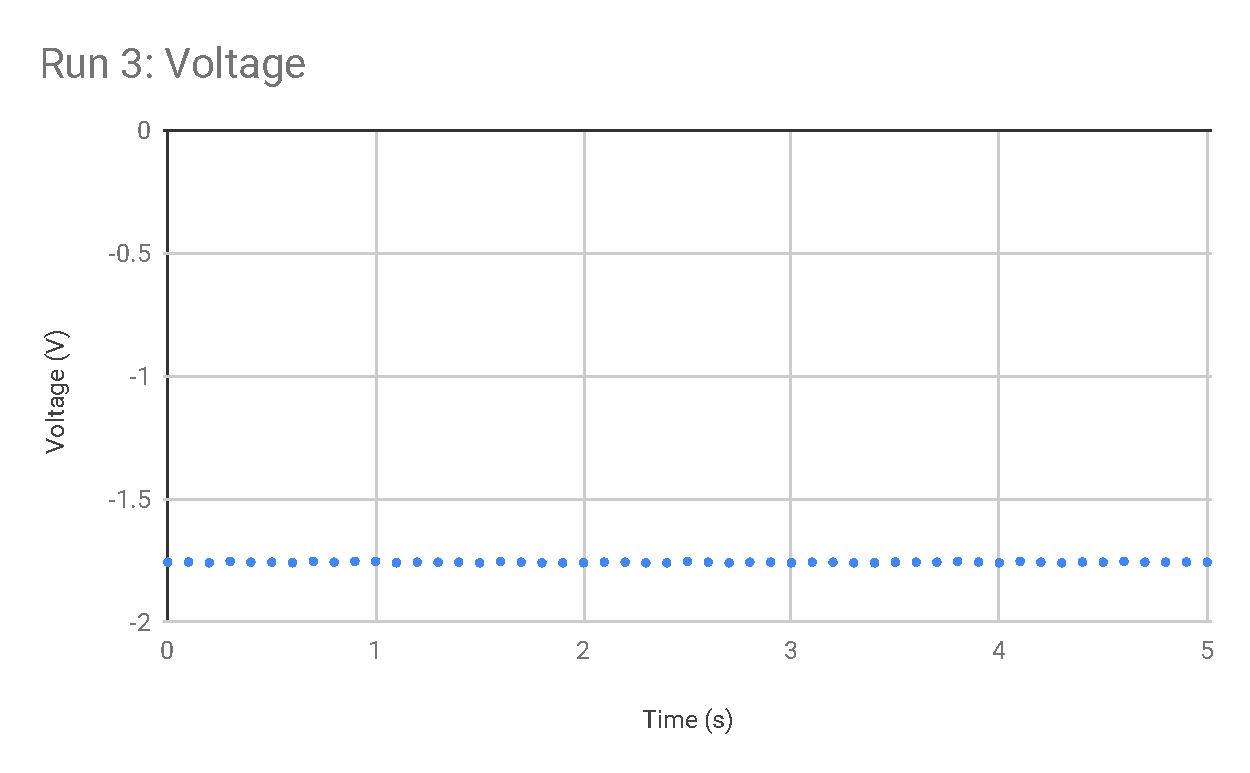
\includegraphics[scale=0.74]{image/03-serial-parallel/resistor-V.pdf}
	\caption{Voltage across ohmic resistor}
	\label{figure.03.resistor.v}
\end{figure}
%
\begin{figure}[ht]
	\centering
	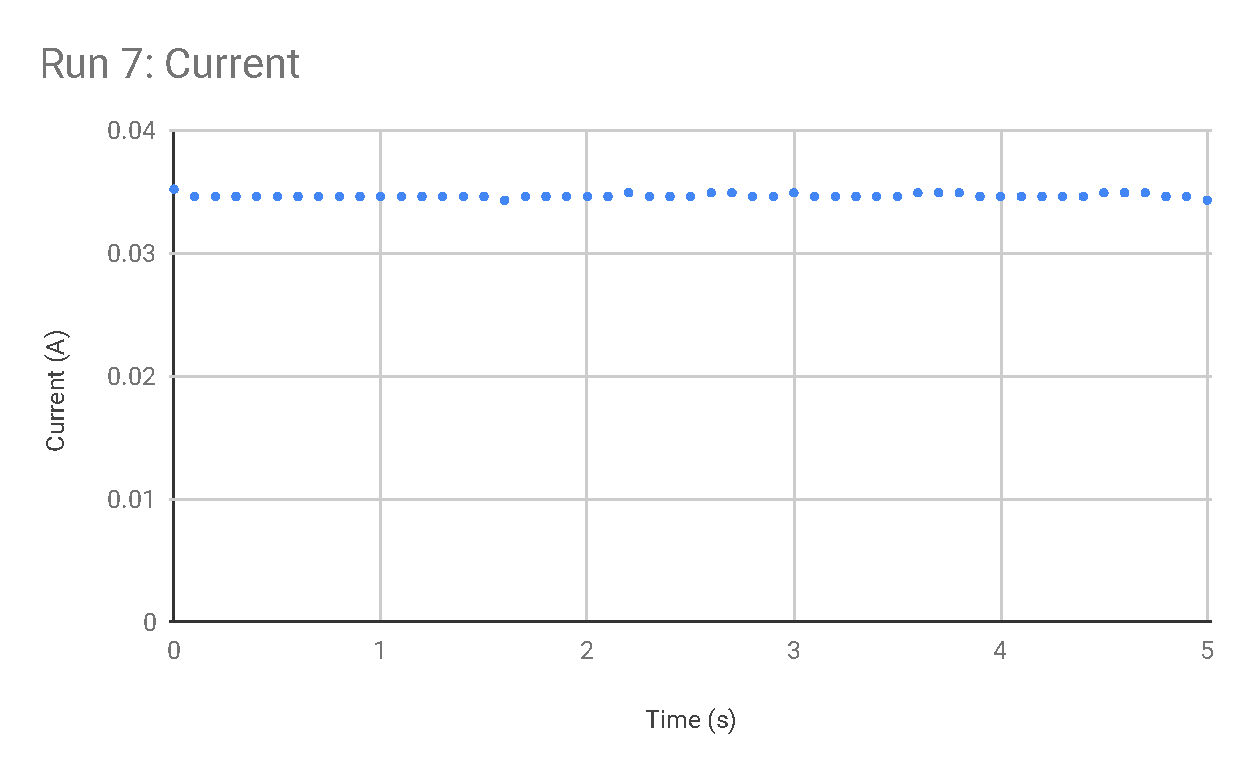
\includegraphics[scale=0.74]{image/03-serial-parallel/resistor-I.pdf}
	\caption{Current through ohmic resistor}
	\label{figure.03.resistor.i}
\end{figure}
%
\begin{figure}[ht]
	\centering
	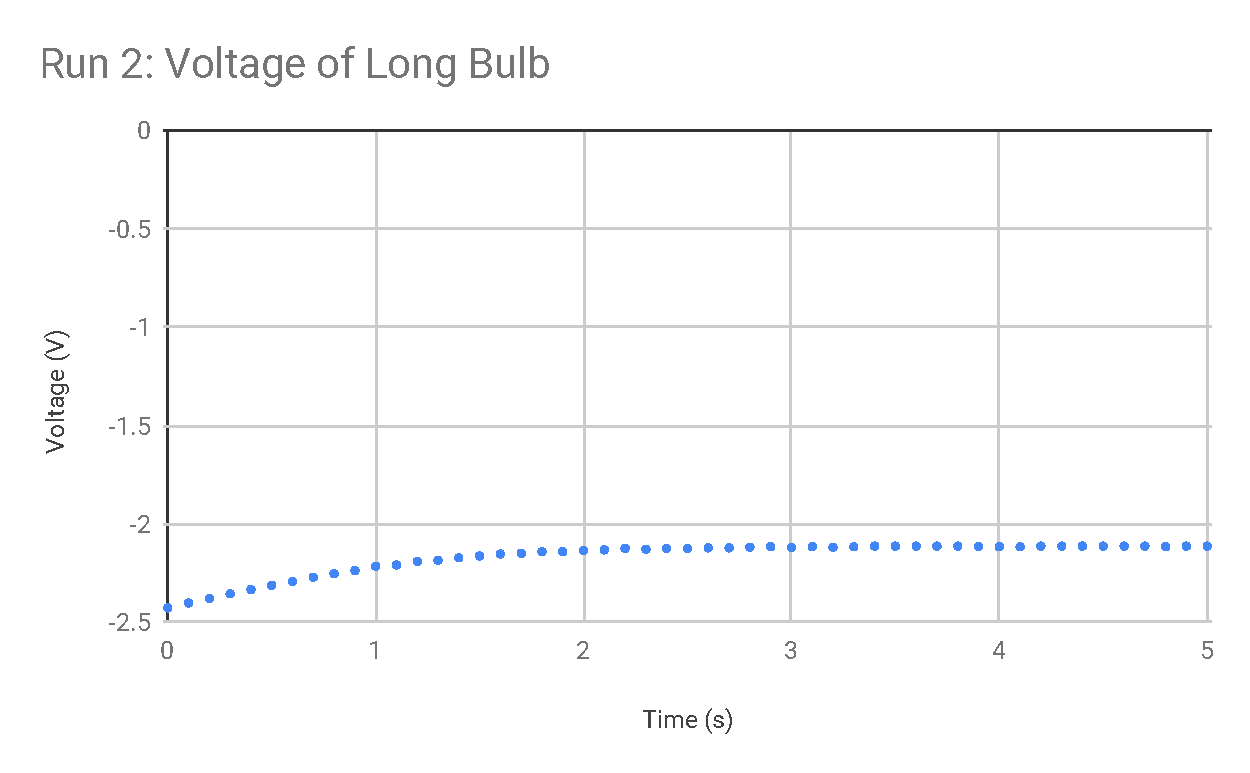
\includegraphics[scale=0.74]{image/03-serial-parallel/bulb-V.pdf}
	\caption{Voltage across non-ohmic light bulb}
	\label{figure.03.bulb.v}
\end{figure}
%
\begin{figure}[ht]
	\centering
	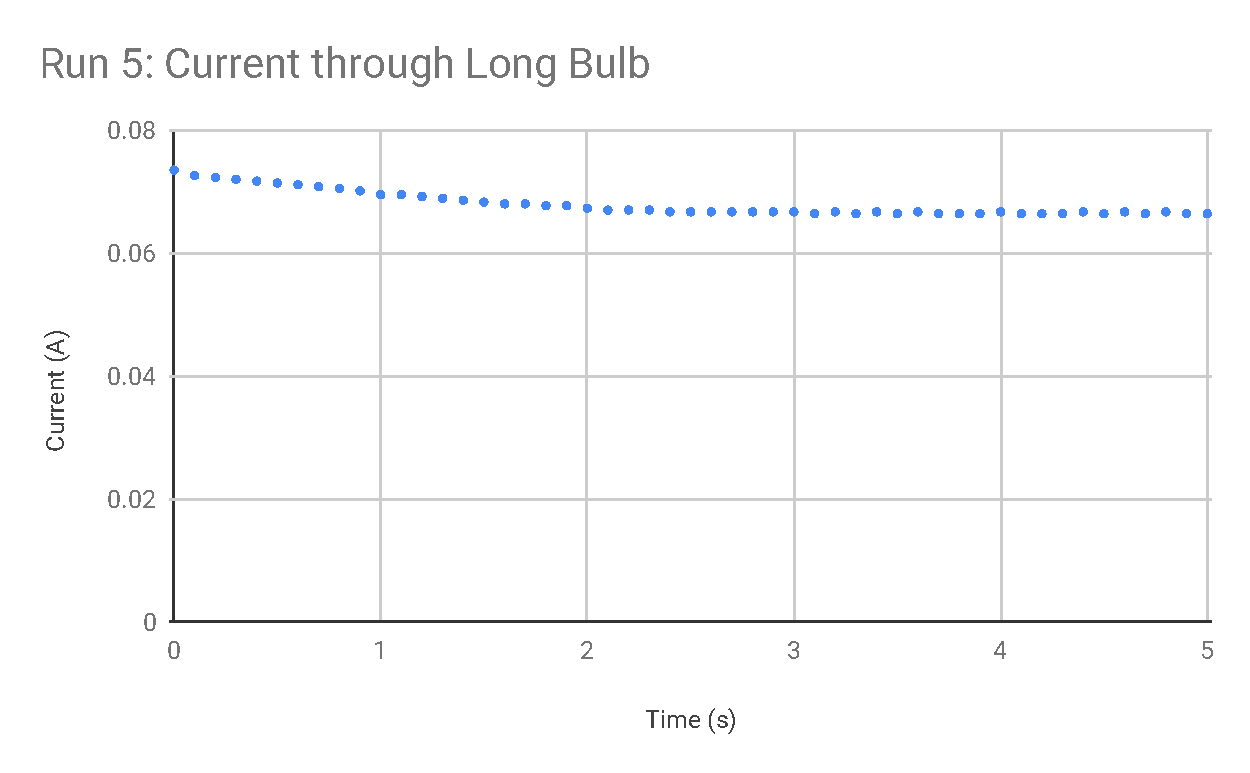
\includegraphics[scale=0.74]{image/03-serial-parallel/bulb-I.pdf}
	\caption{Current through non-ohmic light bulb}
	\label{figure.03.bulb.i}
\end{figure}